\documentclass{article}
\usepackage{amsthm,amsmath,amssymb}
\usepackage{graphicx}
\usepackage{fancyhdr}

\pagestyle{fancy}
\fancypagestyle{firstpage}{%
  \lhead{Research Report, Seong-Eun Cho}
  \rhead{12/5/2017}
}

\begin{document}
\thispagestyle{firstpage}
\raggedright
Application to Cherry's Problem (355) states that  ${\dot{x_1}} = {x_2}, \quad {\dot{x_2}} = {-{\Phi}(x)}$,
which is equivalent to ${\ddot{x}} + {\Phi}(x) = 0$.

First, we let ${\Phi}(x) = sin(x)$ and we obtain the phase portrait below:
\linebreak

\centering
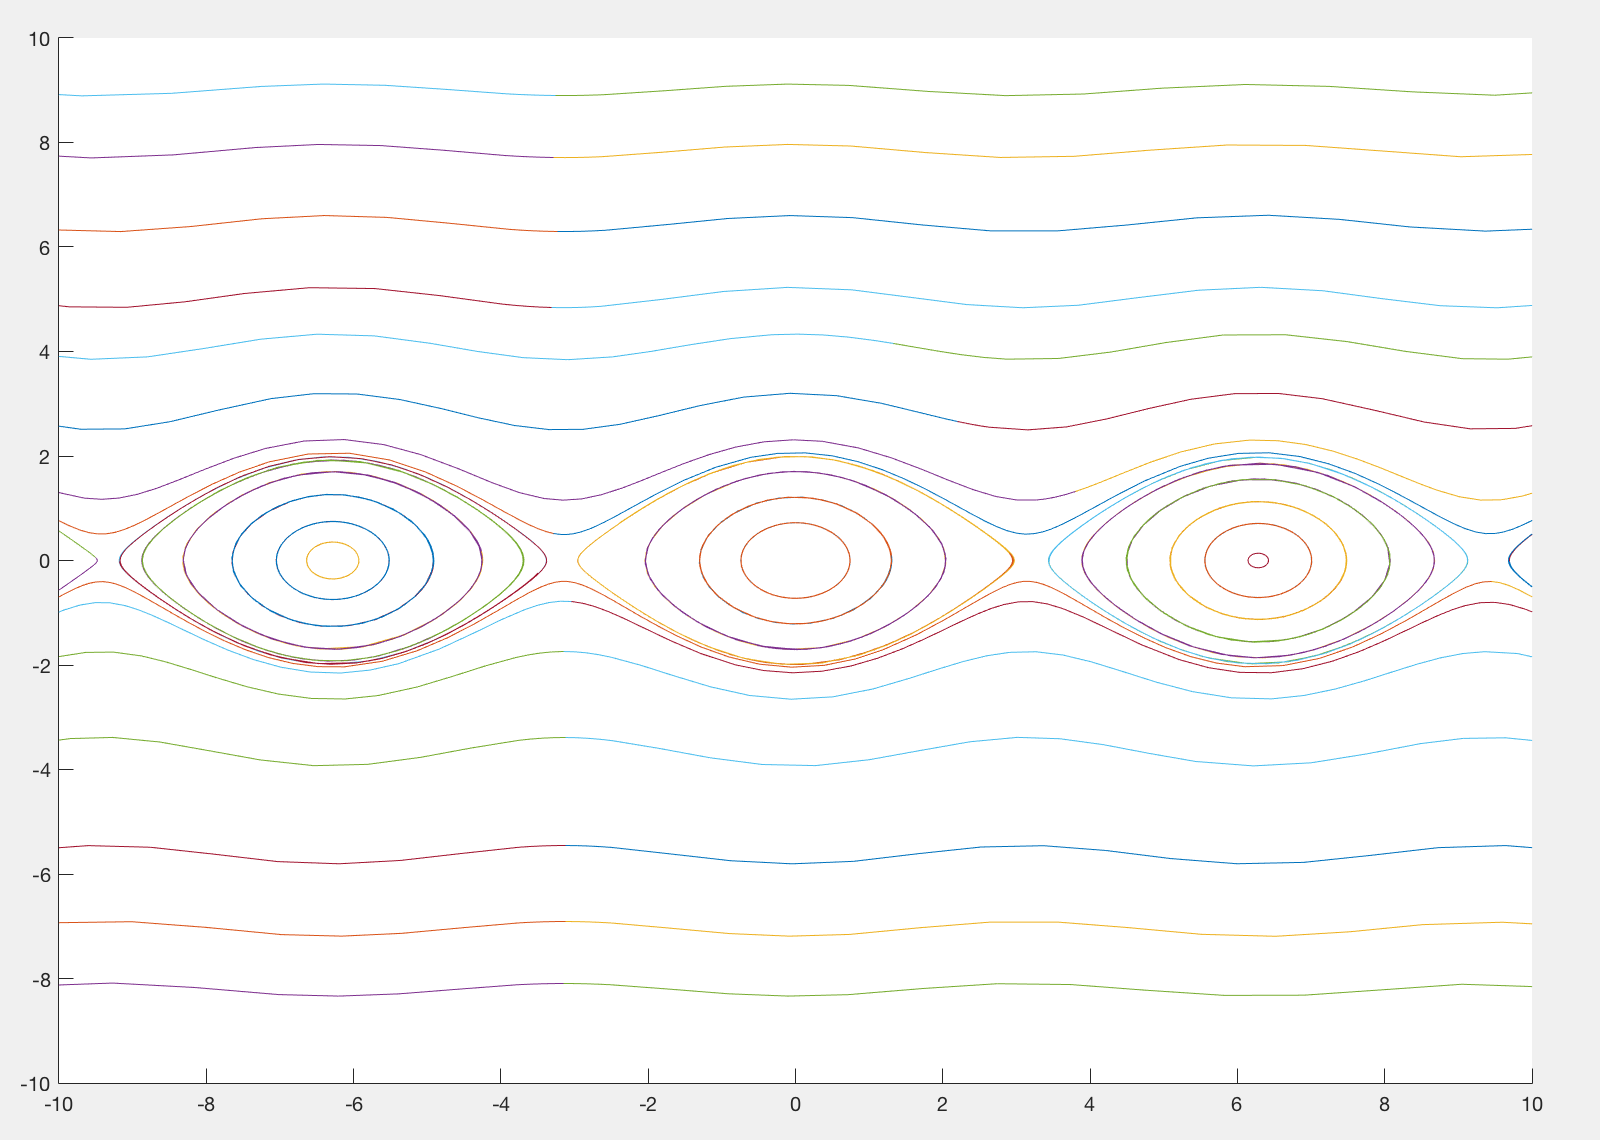
\includegraphics[width=3in]{sin_x.png}
\linebreak

\raggedright
From the phase portrait, we can observe that every $(k{\pi},0), k \in \mathbb{Z}$, is a critical point. More over, every $(2k{\pi}, 0)$ is a center and ${((2k+1)\pi, 0)}$ is a saddle point. This is consistent with Theorem 4.1 (355) which states that the equation has an orbit $(\phi(x), {\phi}\sp{\prime}(x))$ connecting saddle points $({u_1}^-, 0)$ and $({u_1}^+, 0)$.

\vspace{5mm}

Next, we let $\phi(x) = sin(2{\pi}x/T)$ where $T$ is the period of the function to analyze the change in the critical points with the period of $\phi(x)$ changing. Letting $T = 2$, we get $\phi(x) = sin({\pi}x)$ and it produces:
\linebreak

\centering
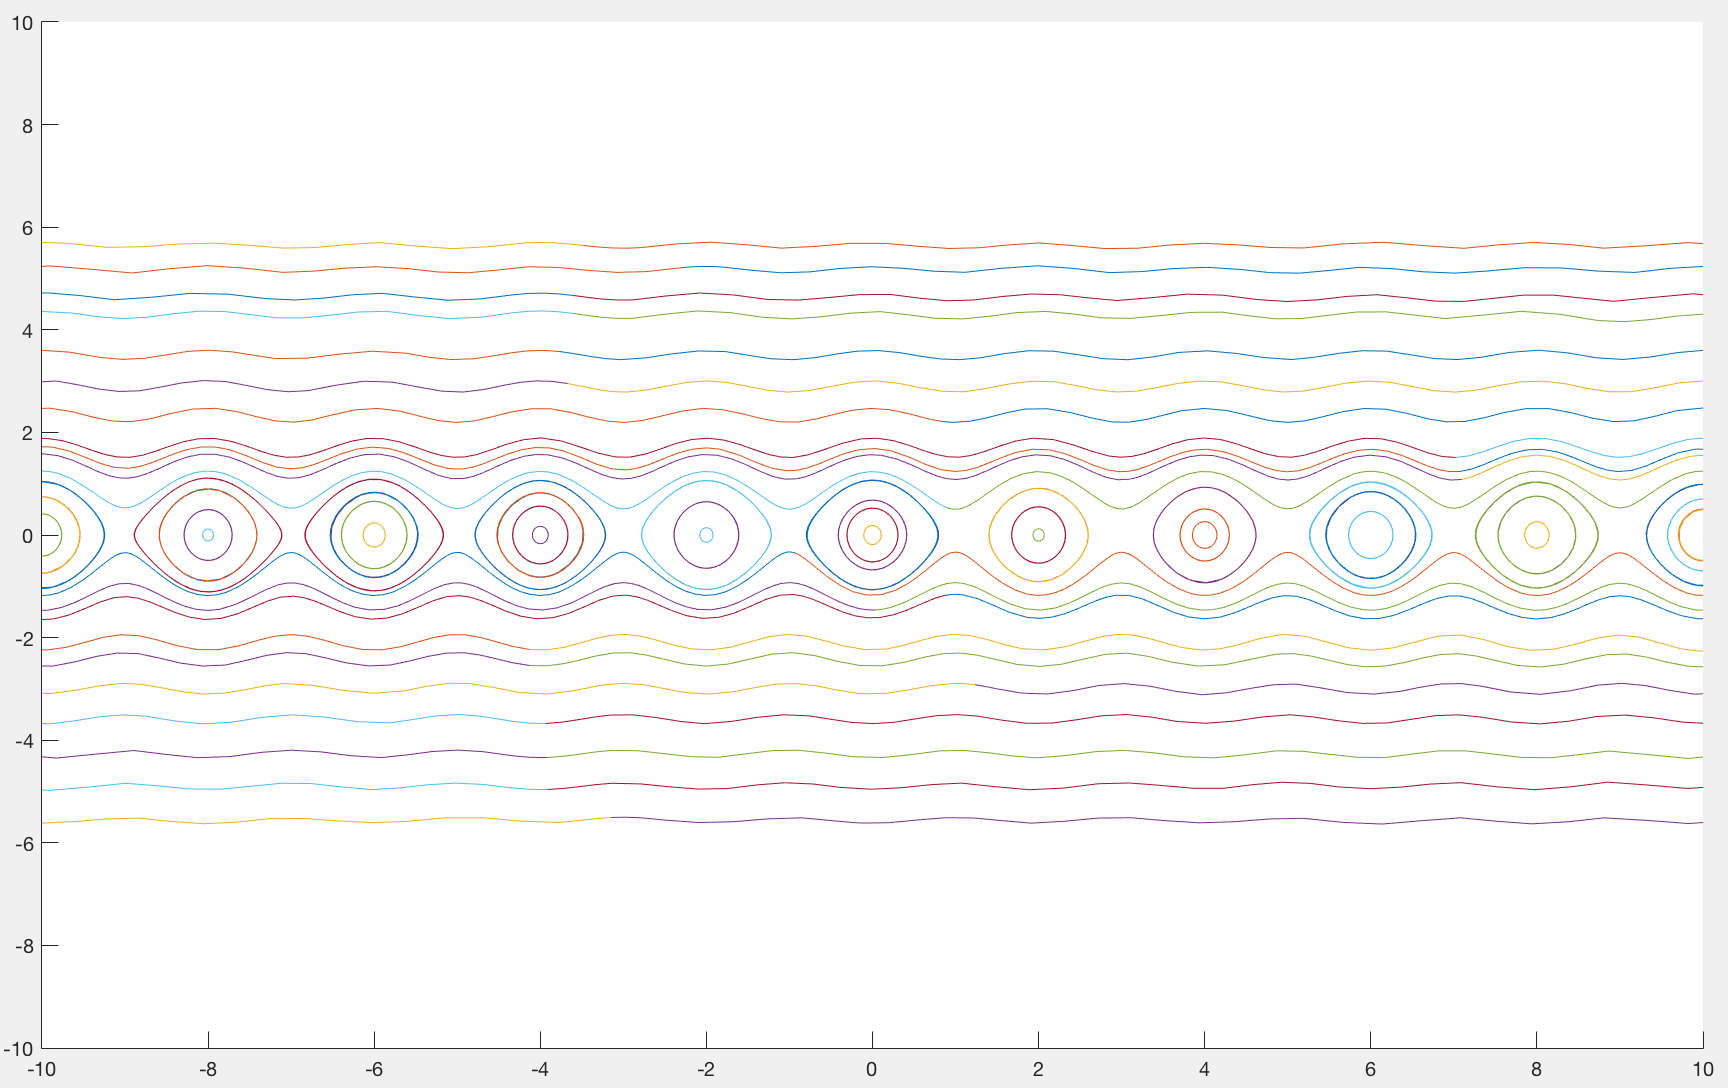
\includegraphics[width=3in]{sin_pi_x.png}
\linebreak

\raggedright
From this diagram, we can see that the critical points change depending on the period of the function. It seems that the center points lie at $(kT, 0), k \in \mathbb{Z}$, and the saddle points at $((2k+1){T/2}, 0)$. 

\newpage
We now let $\phi(x) = cos(x)$. We then obtain:
\linebreak

\centering
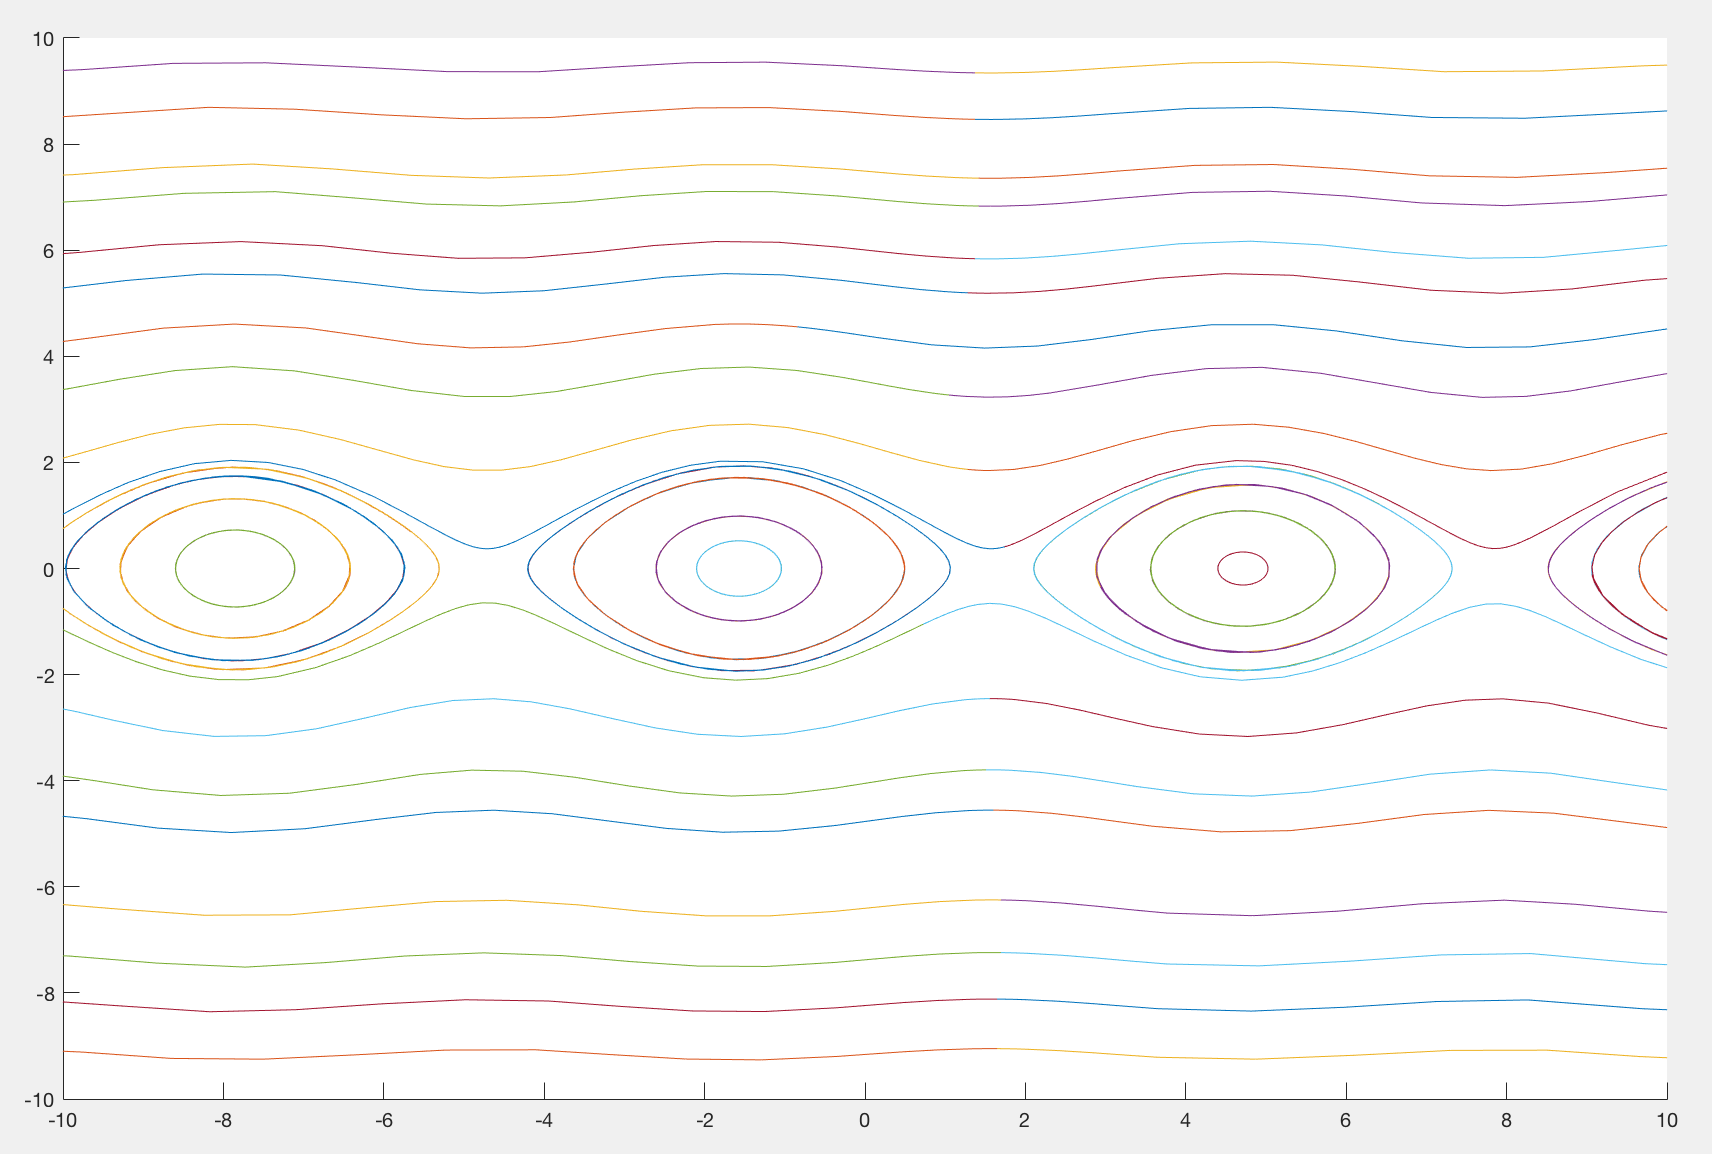
\includegraphics[width=3in]{cos_x.png}
\linebreak

\raggedright
Comparing it to $\phi(x) = sin(x)$, we can see that the the phase portrait shifted $\pi/2$ in the negative direction. Since $cos(x) = sin(x - \pi/2)$, this makes sense. 

\vspace{5mm}

We now choose a different T-periodic function, and see if it acts as we would expect it. We let $\phi(x)$ be defined piecewise as
\linebreak

\centering
$
\phi(x) = 
\left\{
    \begin{array}{ll}
        1 & \quad x \in (0, \pi) \\
        -1 & \quad x \in (\pi, 2\pi) \\
        0 & \quad x = 0 \\
    \end{array}
\right.
$
\linebreak

\raggedright
and $\phi(x + T) = \phi(x)$, with $T = 2\pi$ in this case. 

\vspace{5mm}
\centering
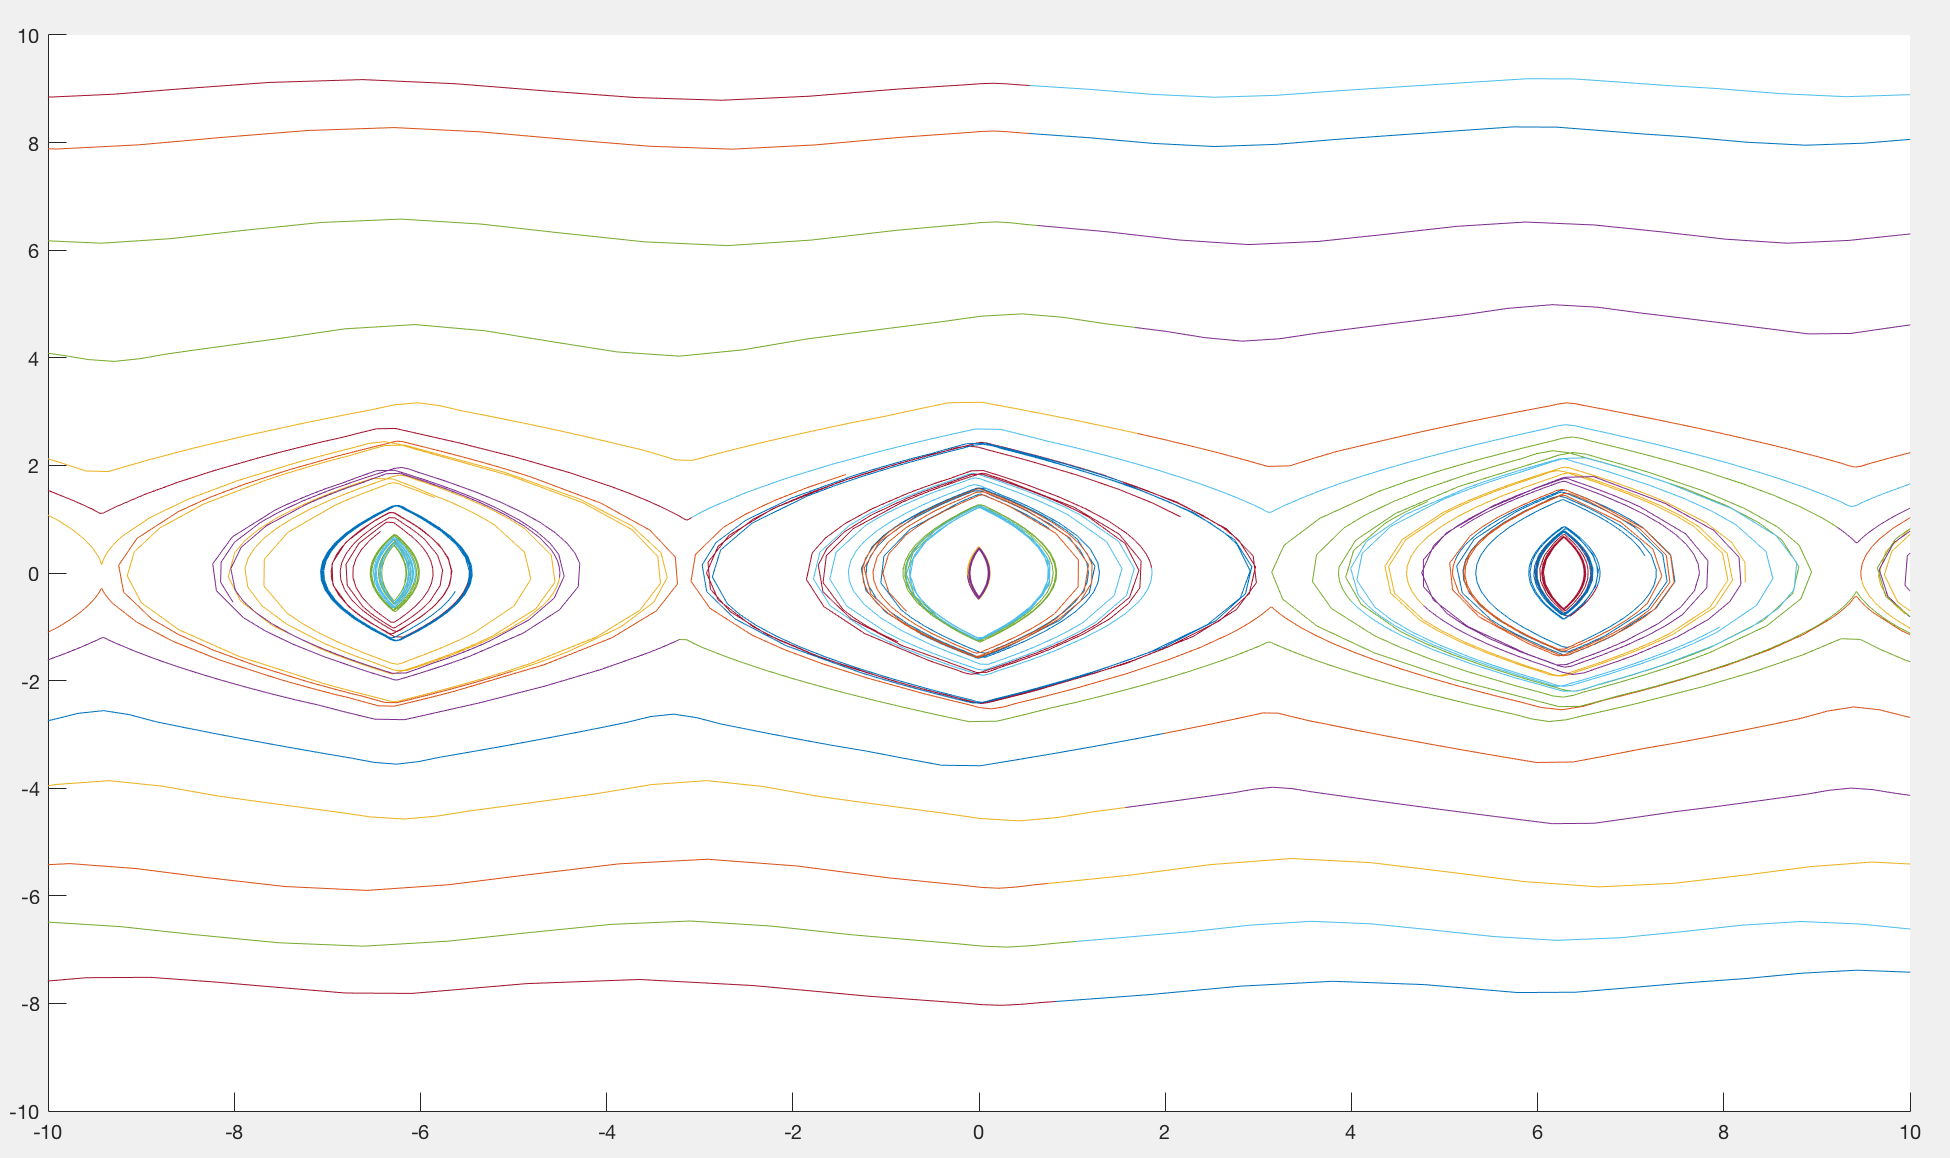
\includegraphics[width=3in]{piecewise.png}
\linebreak

\raggedright
Although this function is not continuous, it can still be transformed as a Fourier series. We see that the key characteristics of its critical points remain the same as when $\phi(x) = sin(x)$

\newpage
We now look at system of equations ${\dot{x_1}} = {x_2}, \quad {\dot{x_2}} = -{\lambda}p(t)\Phi(x)$, which is equivalent to ${\ddot{x}} + {\lambda}p(t)\Phi(x) = 0$.

We let ${\lambda}p(t) = t$ and $\phi(x) = sin(x)$ and it produces the phase portrait below:
\linebreak

\centering
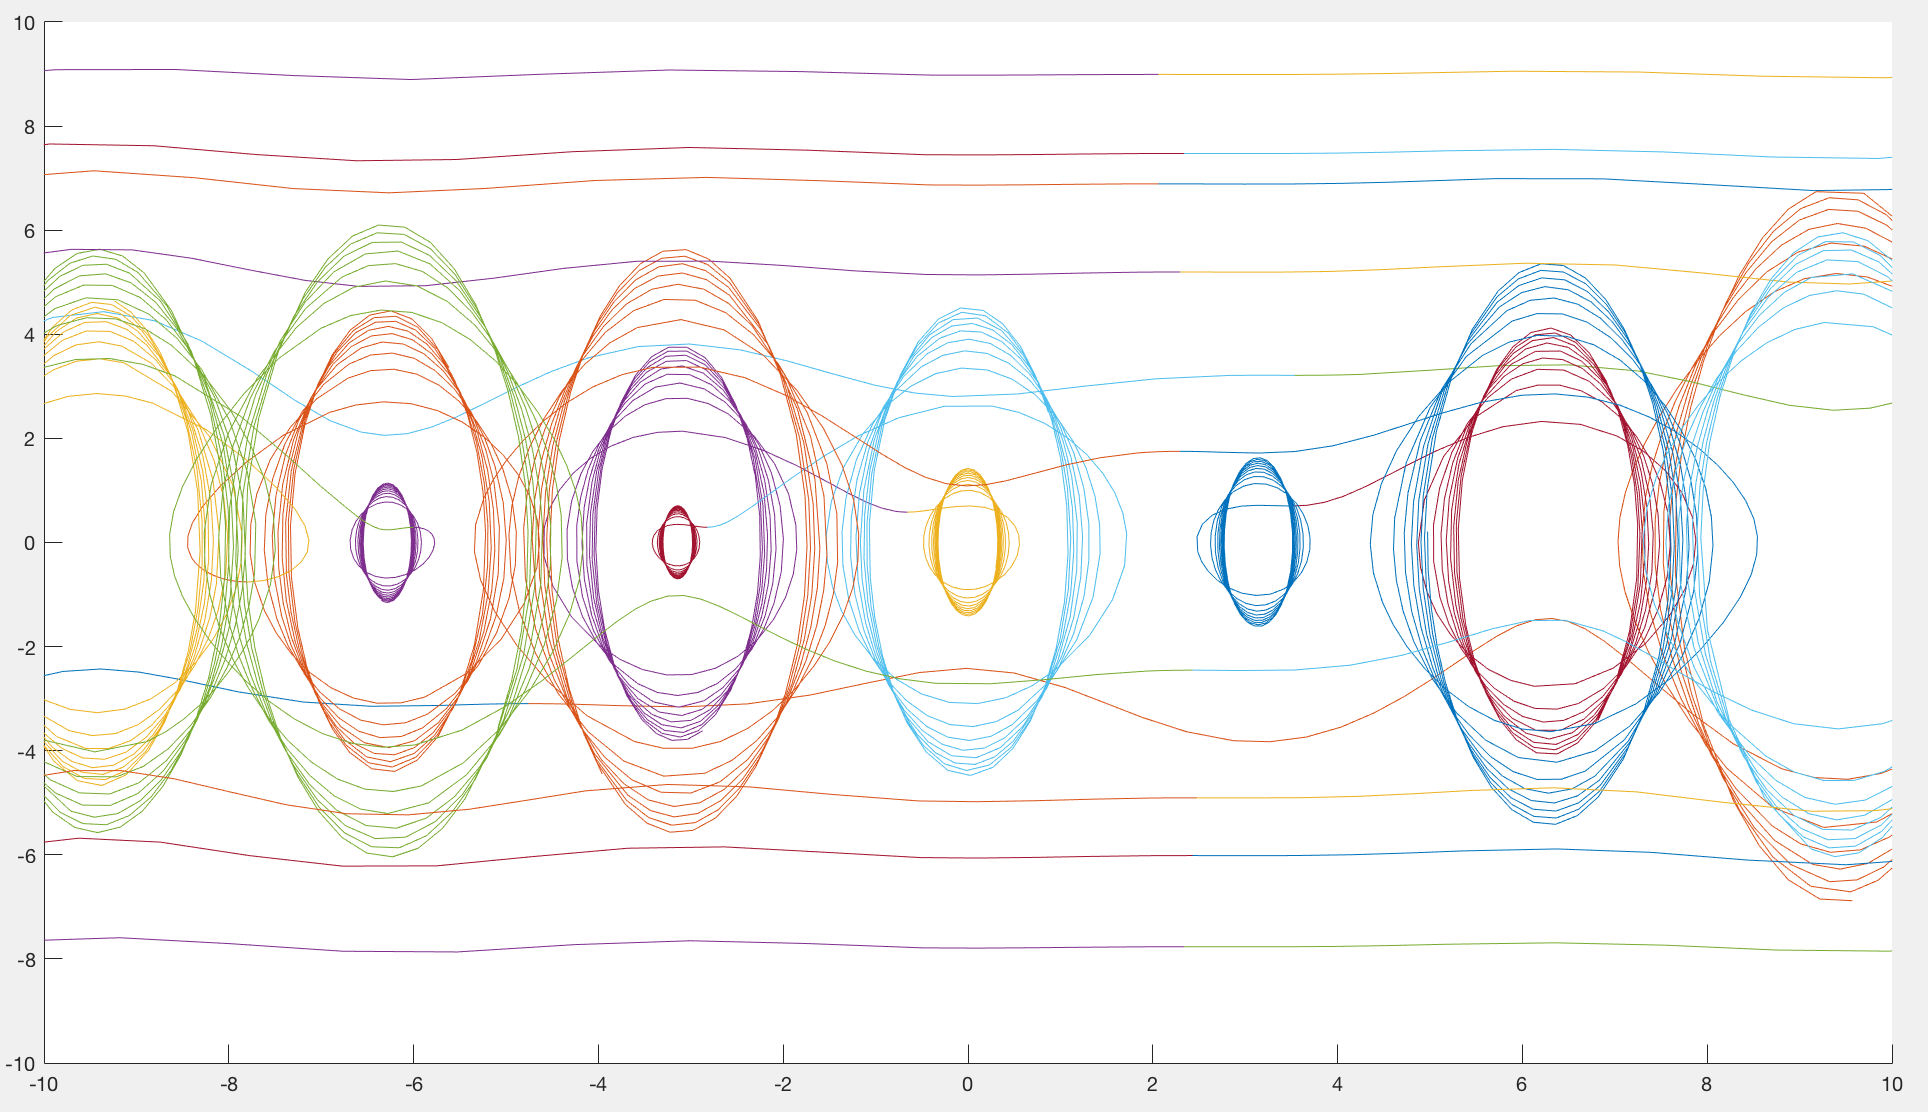
\includegraphics[width=3in]{t_sin_x.png}
\linebreak

\raggedright
From this portrait, I'm not completely sure if the portrait I produced is correct, or if I made a mistake when adding a new function of $t$. It almost seems as though the graph should be visualized with 3 dimensions. 

\end{document}
